\section{Servidor na nuvem}

\subsection{Descrição}

O servidor na nuvem é composto por um servidor WebSocket para comunicação entre clientes e casas, um banco de dados em memória para armazenar informações sobre conexões WebSocket ativas, uma API REST para acesso aos dados persistidos, um banco de dados não-relacional para armazenar dados dos sensores, módulos, Morpheus e usuários, um proxy reverso e um firewall.

Para fins de prova de conceito, optou-se por prosseguir com uma arquitetura monolítica. A implementação da arquitetura de microsserviços aumentaria consideravelmente a complexidade do projeto, e seus principais benefícios não seriam tão bem aproveitados, visto que o sistema não seria colocado a provas de carga real no momento. Contudo, ressalta-se que o monolito que compõe o servidor na nuvem poderia sim ser implementado como um conjunto de microsserviços, o que seria uma evolução natural à medida que o sistema escala.

\subsection{Requisitos}

\subsubsection{Requisitos funcionais}
\begin{description}

\item \textbf{Comunicação}

\begin{itemize}
\item O servidor deve permitir que Morpheus e aplicativos clientes se comuniquem via WebSocket.
\item Morpheus podem enviar as mensagens provenientes dos módulos físicos, que são: configuration, confirmation e data. Também podem receber mensagens destinadas aos módulos físicos, que são: action, configuration e data.
\item Morpheus podem receber mensagens de registro e remoção de módulo para definir quais dispositivos ele gerencia.
\item Morpheus podem enviar mensagens de report.
\item Os aplicativos cliente podem enviar as mensagens correspondentes a interações do usuário, que são: action e configuration. Também podem receber mensagens provenientes dos módulos físicos, que são: confirmation e data.
\item Aplicativos cliente podem receber mensagens de report.
\item Aplicativos cliente podem receber o status de conectividade dos Morpheus e receber notificações quando um Morpheus for desconectado.
\end{itemize}

\item \textbf{Persistência de dados}

\begin{itemize}
\item O servidor deve persistir dados de usuário, de configurações de Morpheus e módulo e de mensagens de dados (data e report).
\end{itemize}

\item \textbf{Gerenciamento de dados}

\begin{itemize}
\item O servidor deve oferecer uma API REST para leitura e escrita de dados de usuário, configurações de Morpheus e de módulos.
\end{itemize}

\end{description}

\subsubsection{Requisitos não-funcionais}

\begin{itemize}
\item O servidor deve permitir o estabelecimento de conexões HTTPS seguras e criptografadas.
\item O firewall deve bloquear conexões em portas que não estão sendo utilizadas.
\end{itemize}

\subsection{Tecnologias usadas}

O servidor foi desenvolvido usando Node.js \footnote{https://nodejs.org}, um ambiente em tempo de execução para código em JavaScript. Sua arquitetura usa um modelo orientado a eventos e realiza a execução de comandos concorrentemente sem bloquear o servidor. Assim, servidores em Node.js conseguem alcançar uma melhor escalabilidade, suportando múltiplas conexões simultâneas sem impactos de performance.

Para a persistência de dados, foi escolhido o MongoDB \footnote{https://www.mongodb.com/}, banco de dados não-relacional baseado em documentos. A facilidade de integração com JavaScript e Node.js, a similaridade dos documentos com objetos JSON e a natureza dos dados de sensores foram as motivações para sua escolha como banco de dados principal.

Contudo, não são apenas informações sobre usuários e dispositivos e dados coletados pelos sensores que precisam ser armazenados. Para gerenciar quais Morpheus estão conectados à nuvem e e a quais aplicativos suas informações em tempo real devem ser enviadas, é usado o Redis \footnote{https://redis.io/}, banco de dados em memória. Redis é popularmente usado para fins como cache, mensageria e implementação de filas. No caso do Hedwig, ele é utilizado para armazenar informações de sessão, que são temporárias e requerem baixas latências para leitura e escrita.

Para implementar a comunicação entre aplicativos e casas, foi escolhida a biblioteca Socket.io \footnote{https://socket.io/}, que fornece uma API de alto nível para troca de informações bidirecional por meio de eventos. Além de abstrair a API de baixo nível do protocolo de WebSockets, o Socket.io já fornece eventos referentes ao status da conexão, facilitando o disparo de notificações caso o controlador de uma casa seja desconectado, e implementa um fallback para clientes que não suportam o protocolo de WebSocket. Por exemplo, se um usuário acessa um aplicativo por meio de um navegador antigo, a troca de dados continua sendo feita por meio de long polling.

A arquitetura possui um proxy reverso que é responsável por enviar as requisições ao servidor em Node.js. Para isso, foi usado o nginx \footnote{https://nginx.org/}, popularmente utilizado como servidor HTTP e proxy genérico para TCP e UDP. Ele permite a configuração de conexões seguras via HTTPS e dispensa a necessidade de delegar privilégios para acessar as portas reservadas 80 e 443 ao processo que roda o servidor Node.js.

Por fim, foi usada a ferramenta padrão do Ubuntu para firewall, ufw, que permite criar regras para bloquear tráfego IPv4 e IPv6.

\begin{figure}[H]
	\centering
	\caption{Componentes e implementação na nuvem}
  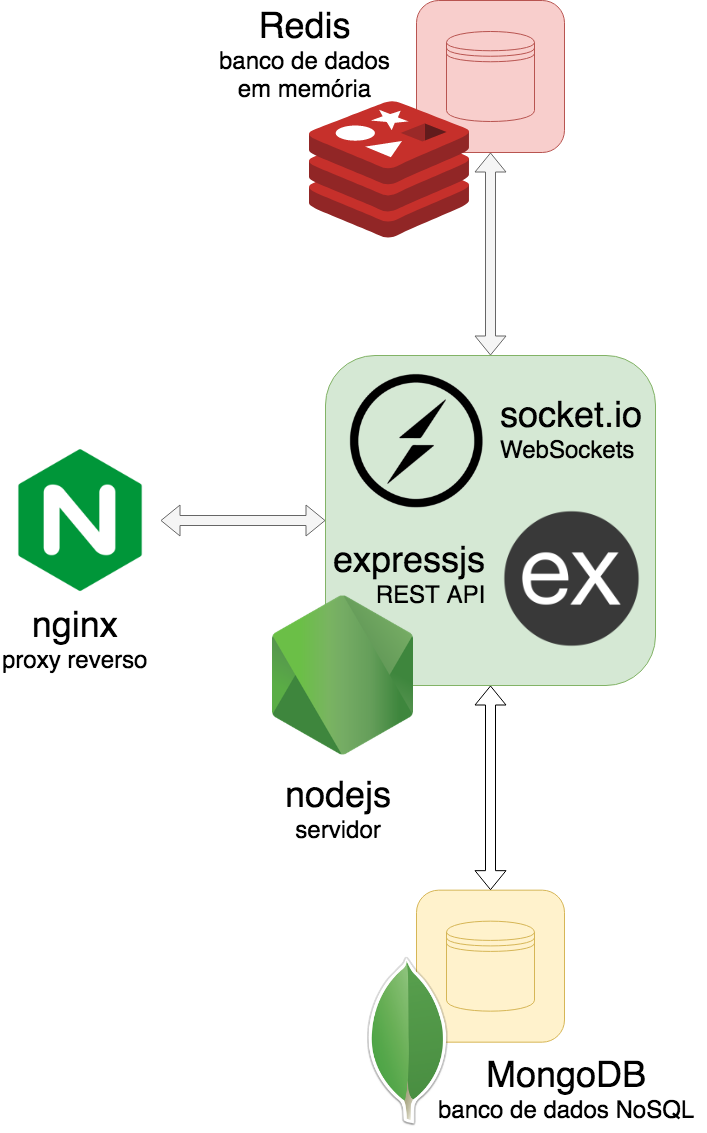
\includegraphics[width=0.5\textwidth]{componentesNuvem}
\label{fig:componentesNuvem}
\end{figure}

\subsection{Infraestrutura}

Para hospedar o servidor do Hedwig, foi utilizado o serviço de computação na nuvem Digital Ocean \footnote{https://www.digitalocean.com/}. Com ele, foi possível implantar o servidor em uma instância que roda Ubuntu 16.04.3 x64, com 1 CPU, 512MB de memória, 20GB de armazenamento de disco SSD e 1000GB de cota disponível para transferência de dados. O data center que hospeda essa instância fica em Nova Iorque.
